\documentclass{beamer}

\usepackage{beamerthemesplit}
\usepackage{graphicx}
\usepackage{color, natbib, hyperref}
\usepackage{bibentry}
\nobibliography*

% define colors
\definecolor{jblue}  {RGB}{20,50,100}
\definecolor{ngreen} {RGB}{98,158,31}

%theme

\usetheme{boxes} 
%\usecolortheme{seahorse} 
\setbeamertemplate{items}[default] 
%\setbeamercovered{transparent}
\setbeamertemplate{blocks}[rounded]
\setbeamertemplate{navigation symbols}{} 
% set the basic colors
\setbeamercolor{palette primary}   {fg=black,bg=white}
\setbeamercolor{palette secondary} {fg=black,bg=white}
\setbeamercolor{palette tertiary}  {bg=jblue,fg=white}
\setbeamercolor{palette quaternary}{fg=black,bg=white}
\setbeamercolor{structure}{fg=jblue}
\setbeamercolor{titlelike}         {bg=jblue,fg=white}
\setbeamercolor{frametitle}        {bg=jblue!10,fg=jblue}
\setbeamercolor{cboxb}{fg=black,bg=jblue}
\setbeamercolor{cboxr}{fg=black,bg=red}

% reduce space before/after equations
\expandafter\def\expandafter\normalsize\expandafter{%
    \normalsize
    \setlength\abovedisplayskip{1pt}
    \setlength\belowdisplayskip{1pt}
    \setlength\abovedisplayshortskip{1pt}
    \setlength\belowdisplayshortskip{1pt}
}

% set colors for itemize/enumerate
\setbeamercolor{item}{fg=ngreen}
\setbeamercolor{item projected}{fg=white,bg=ngreen}

% set colors for blocks
\setbeamercolor{block title}{fg=ngreen,bg=white}
\setbeamercolor{block body}{fg=black,bg=jblue!10}

% set colors for alerted blocks (blocks with frame)
\setbeamercolor{block alerted title}{fg=white,bg=jblue}
\setbeamercolor{block alerted body}{fg=black,bg=jblue!10}
\setbeamercolor{block alerted title}{fg=white,bg=dblue!70} % Colors of the highlighted block titles
\setbeamercolor{block alerted body}{fg=black,bg=dblue!10} % Colors of the body of highlighted blocks

% set the fonts
\usefonttheme{professionalfonts}

\setbeamerfont{section in head/foot}{series=\bfseries}
\setbeamerfont{block title}{series=\bfseries}
\setbeamerfont{block alerted title}{series=\bfseries}
\setbeamerfont{frametitle}{series=\bfseries}
\setbeamerfont{frametitle}{size=\Large}
\setbeamerfont{block body}{series=\mdseries}
\setbeamerfont{caption}{series=\mdseries}
\setbeamerfont{headline}{series=\mdseries}


% set some beamer theme options
\setbeamertemplate{title page}[default][colsep=-4bp,rounded=true]
\setbeamertemplate{sections/subsections in toc}[square]
\setbeamertemplate{items}[circle]
\setbeamertemplate{blocks}[width=0.0]
\beamertemplatenavigationsymbolsempty

% Making a DAG
\usepackage{tkz-graph}  
\usetikzlibrary{shapes.geometric}
\tikzstyle{VertexStyle} = [shape            = ellipse,
                               minimum width    = 6ex,%
                               draw]
 \tikzstyle{EdgeStyle}   = [->,>=stealth']      


% Math macros
\newcommand{\cD}{{\mathcal D}}
\newcommand{\cF}{{\mathcal F}}
\newcommand{\todo}[1]{{\color{red}{TO DO: \sc #1}}}

\newcommand{\reals}{\mathbb{R}}
\newcommand{\integers}{\mathbb{Z}}
\newcommand{\naturals}{\mathbb{N}}
\newcommand{\rationals}{\mathbb{Q}}

\newcommand{\ind}[1]{1_{#1}} % Indicator function
\newcommand{\pr}{\mathbb{P}} % Generic probability
\newcommand{\ex}{\mathbb{E}} % Generic expectation
\newcommand{\var}{\textrm{Var}}
\newcommand{\cov}{\textrm{Cov}}

\newcommand{\normal}{N} % for normal distribution (can probably skip this)
\newcommand{\eps}{\varepsilon}
\newcommand\independent{\protect\mathpalette{\protect\independenT}{\perp}}
\def\independenT#1#2{\mathrel{\rlap{$#1#2$}\mkern2mu{#1#2}}}

\newcommand{\convd}{\stackrel{d}{\longrightarrow}} % convergence in distribution/law/measure
\newcommand{\convp}{\stackrel{P}{\longrightarrow}} % convergence in probability
\newcommand{\convas}{\stackrel{\textrm{a.s.}}{\longrightarrow}} % convergence almost surely

\newcommand{\eqd}{\stackrel{d}{=}} % equal in distribution/law/measure
\newcommand{\argmax}{\arg\!\max}
\newcommand{\argmin}{\arg\!\min}


\mode<presentation>

\title[Model-based matching]{Model-based matching for causal inference in observational studies}
\author{Kellie Ottoboni \\ with Philip B. Stark and Jasjeet Sekhon}
\institute[]{Department of Statistics, UC Berkeley\\Berkeley Institute for Data Science}
\date{March 15, 2016}

\begin{document}

\frame{\titlepage}

\AtBeginSection[]
{
   \begin{frame}
       \frametitle{Outline}
       \tableofcontents[currentsection]
   \end{frame}
}



\section[Introduction]{Introduction}
\frame
{
  \frametitle{Observational Studies vs Experiments}
 \begin{center}
\begin{itemize}
\item \textbf{Problem:} Estimate the causal effect of a treatment on outcome of interest
\item In randomized experiments, treatment is assigned to individuals at random.
\item In observational studies, the way individuals select into treatment groups is unknown.
%\item \textbf{Confounding} occurs when a variable affects both treatment assignment and the outcome. It biases our estimates of the treatment effect.
\end{itemize}

\begin{figure}[h]
\begin{tikzpicture}
\SetGraphUnit{2} 
\Vertex{Outcome} \NOWE(Outcome){Treatment} \NOEA(Outcome){Confounder}
\Edges[color=red, label=?](Treatment, Outcome) \Edges(Confounder, Outcome) \pause \Edges(Confounder, Treatment) 
\end{tikzpicture}
\end{figure}
\end{center}
}


\frame{
\frametitle{Motivating Example: Toads and Packstock}
\begin{figure}[htbp]
\begin{center}
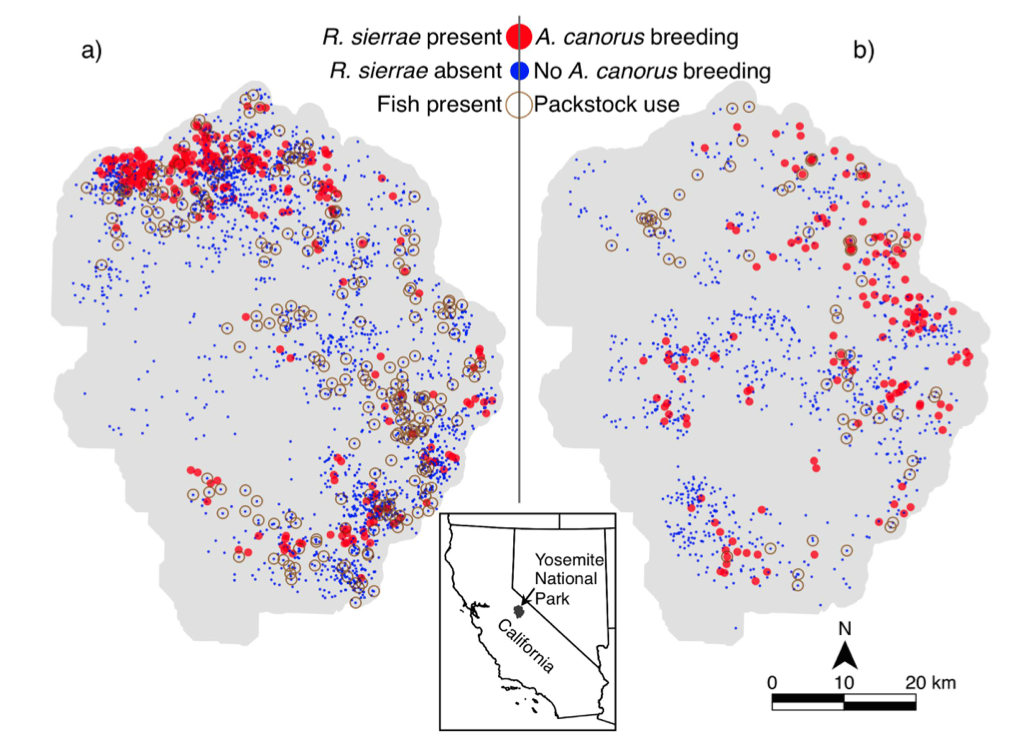
\includegraphics[height = 0.75\textheight]{fig/toadmap.png}
\end{center}
\end{figure}


\tiny
J. R. Matchett, Philip B. Stark, Steven M. Ostoja, Roland A. Knapp, Heather C. McKenny, Matthew L. Brooks,
William T. Langford, Lucas N. Joppa, and Eric L. Berlow. Detecting the influence of rare stressors on rare species in Yosemite National Park using a novel stratified permutation test.
Scientific Reports, 5: 10702, June 2015.
}

\frame{
\frametitle{Motivating Example: Toads and Packstock}
\begin{itemize}
\itemsep10pt
\item The response is rare (few meadows have toads).
\item The treatment is rare (few meadows are used by packstock).
\item Randomized experiment is impossible, and toad/packstock presence is not random across meadows.
\item We're interested in detecting any effect, no matter how small. If treatment effect varies across meadows, then averages might not be informative.
\end{itemize}
}





\frame{
\frametitle{Neyman-Rubin Causal Model}
\begin{center}
\begin{itemize}

\item Population of $i = 1, \dots, N$ individuals. Each individual has two \textbf{potential outcomes}.
\item $Y_i(1)$ is individual $i$'s outcome if he receives treatment
\item $Y_i(0)$ is individual $i$'s outcome if he is in the control group
\item The treatment effect for individual $i$ is $\tau_i = Y_i(1) - Y_i(0)$
\end{itemize}
\end{center}
\vspace{50pt}

\begin{center}
\begin{tikzpicture}[overlay, remember picture]
\centering
\draw (-2.5,0) rectangle (-1.5,1) node[pos=.5] {$Y_2(1)$};\draw (-1.5,0) rectangle (-0.5,1)node[pos=.5] {$Y_2(0)$};
\draw (-2.5,1.5) rectangle (-1.5,2.5) node[pos=.5] {$Y_1(1)$}; \draw (-1.5,1.5) rectangle (-0.5,2.5) node[pos=.5] {$Y_1(0)$};
\draw (0.5,0) rectangle (1.5,1) node[pos=.5] {$Y_4(1)$}; \draw (1.5,0) rectangle (2.5,1) node[pos=.5] {$Y_4(0)$};
\draw (0.5,1.5) rectangle (1.5,2.5) node[pos=.5] {$Y_3(1)$}; \draw (1.5,1.5) rectangle (2.5,2.5) node[pos=.5] {$Y_3(0)$};
\end{tikzpicture}

\end{center}
}

\frame{
\frametitle{Fundamental Problem of Causal Inference \small{\citep{holland_statistics_1986}}}
\begin{center}
\begin{itemize}
\item We may never observe both $Y_i(1)$ and $Y_i(0)$
\item $T_i$ is a treatment indicator: $1$ if $i$ is treated, $0$ if $i$ is control
\item The observed outcome for individual $i$ is $Y_i = T_iY_i(1) + (1-T_i)Y_i(0)$
\end{itemize}
\end{center}

\vspace{50pt}

\begin{center}
\begin{tikzpicture}[overlay, remember picture]
\centering
\draw (-2.5,0) rectangle (-1.5,1) node[pos=.5] {$Y_2(1)$}; \draw[fill=black]  (-1.5,0) rectangle (-0.5,1)node[pos=.5] {$Y_2(0)$};
\draw (-2.5,1.5) rectangle (-1.5,2.5) node[pos=.5] {$Y_1(1)$}; \draw[fill=black]  (-1.5,1.5) rectangle (-0.5,2.5) node[pos=.5] {$Y_1(0)$};
\draw[fill=black]  (0.5,0) rectangle (1.5,1) node[pos=.5] {$Y_4(1)$}; \draw (1.5,0) rectangle (2.5,1) node[pos=.5] {$Y_4(0)$};
\draw[fill=black]  (0.5,1.5) rectangle (1.5,2.5) node[pos=.5] {$Y_3(1)$}; \draw (1.5,1.5) rectangle (2.5,2.5) node[pos=.5] {$Y_3(0)$};
\end{tikzpicture}
\end{center}

}


\frame{
\frametitle{Goal}
\textbf{Goal:} test the \textbf{strong null hypothesis} of no treatment effect whatsoever. \\

\begin{align*}
H_0&: Y_i(1) = Y_i(0) \text{ for all } i \\
H_1&: Y_i(1) \neq Y_i(0) \text{ for some } i
\end{align*}

\vspace{20pt}
We'd like our test to have power to detect
\begin{itemize}
\item non-constant effects
\item non-linear effects
\item effects with non-constant sign
\end{itemize}

}

\section[Matching]{Matching}



\begin{frame}
  \frametitle<1>{Matching}
  \frametitle<2>{Aside... the curse of dimensionality }

  \begin{overlayarea}{\textwidth}{2cm}
    \only<1>{
	Individuals with similar covariates should have similar outcomes, but for the treatment. \\
	\begin{itemize}
	\item \textbf{Ideal:} group individuals by $X_i$ to estimate subgroup treatment effects and then average over subgroups
	\item \textbf{Reality:} many covariates, perhaps continuous, make it difficult to stratify
	\end{itemize}
	}
    \only<2>{ 
	\begin{itemize}
	\item If $d$ covariates are split into $k$ bins, we have $d^k$ groups.
	\item To guarantee that we have at least one treated and one control in each group with $95\%$ probability, we need
	$$n \geq \frac{2 \log(1 - (0.95)^{1/k^{d+1}})}{\log(\frac{k^d - 1}{k^d})}$$
	\item If $d = 5$ and $k = 2$, $n \geq 225$.\\
	\item If $d = 10$ and $k = 2$, $n \geq 10,844$.
	\end{itemize}
	 }
  \end{overlayarea}
  \vspace{70pt}
    \begin{overlayarea}{\textwidth}{2cm}
    \begin{center}
	\begin{tikzpicture}[scale = 0.5]
		\foreach \x in{0,...,4}
		{   \draw (0,\x ,4) -- (4,\x ,4);
		    \draw (\x ,0,4) -- (\x ,4,4);
    		\draw (4,\x ,4) -- (4,\x ,0);
    		\draw (\x ,4,4) -- (\x ,4,0);
    		\draw (4,0,\x ) -- (4,4,\x );
    		\draw (0,4,\x ) -- (4,4,\x );
		}
	\end{tikzpicture}
    \end{center}
  \end{overlayarea}
\end{frame}





\frame{
\frametitle{Matching}
\begin{center}
\begin{itemize}
\item \textbf{Solution:} use a one-dimensional score to match or group individuals
\end{itemize}
\end{center}
}


\subsection[Propensity score matching]{Propensity score matching}

\frame{
\frametitle{Propensity score matching}
\begin{itemize}
\itemsep20pt
\item The \textbf{propensity score} is an individual's probability of being assigned treatment, conditional on their covariates
$$ p(x) = \mathbb{P}(T = 1 \mid X = x)$$
\item The propensity score is a balancing score: $X \independent T \mid p(X)$
\item For individuals with the same propensity score, treatment assignment is as if random
\end{itemize}
}

\frame{
\frametitle{Propensity score matching}
\begin{theorem}[\cite{rosenbaum_central_1983}]
If treatment assignment is independent of potential outcomes given $X$, 
$$(Y(1), Y(0)) \independent T \mid X$$
 and if every unit has a chance of receiving treatment,
 $$0 < p(X) < 1 \text{ for all }X$$
 then $(Y(1), Y(0)) \independent T \mid p(X)$.
\end{theorem}
In particular, treated units can serve as the counterfactual for controls with the same $p(X)$ 

$$\ex(Y(t) \mid T=1, p(X)) = \ex(Y(t) \mid T=0, p(X)) \text{ for } t = 0,1$$
}

\frame{
\frametitle{Propensity score matching}
This result identifies the average treatment effect in terms of quantities we can estimate:

\begin{align*}
 \ex(Y(1) - Y(0)) &= \ex_{p(x)}\left[ \ex(Y(1) - Y(0) \mid p(x) ) \right] \\
&= \ex_{p(x)}\left[ \ex(Y(1) \mid p(x) ) - \ex(Y(0) \mid p(x) ) \right] \\
&= \ex_{p(x)}\left[ \ex(Y \mid p(x), T=1 )  -\ex(Y \mid p(x), T=0 ) \right] \\
\end{align*}
}



\frame{
\frametitle{Propensity score matching}
$p(x)$ is usually unknown and estimated by $\hat{p}(x)$ using logistic or probit regressions
\begin{itemize}
\item Assumes a simple functional form for relationship between covariates and treatment
\item Assumes that probability of treatment takes same form for all individuals
\item May actually worsen balance if estimated incorrectly \citep{diamond_genetic_2012}
\end{itemize}
\vfill
Matching complicates inference
\begin{itemize}
\item Standard errors are difficult to compute for matching estimators \citep{abadie_large_2006, abadie_failure_2008}
\item Rarely used in hypothesis testing procedures
\item There's no ``optimal'' way to match \citep{austin_comparison_2014}
\end{itemize}

}


\subsection[Model-based matching]{Model-based matching}

\frame{
\frametitle{Model-based Matching}
\textbf{Idea:} Instead of modeling the propensity score, model the outcome \\
\vfill
Computing $\hat{Y}$, the ``best'' prediction of the outcome based on all covariates except for the treatment, buys us two things:

\begin{itemize} 
\item $\hat{Y}$ is a score on which to stratify observations
\item Using residuals $Y-\hat{Y}$ improves precision by removing variation due to $X$ \citep{rosenbaum_covariance_2002}
\end{itemize}
}



\frame{ 
\frametitle{Model-based Matching}
Suppose that outcomes have the form
$$Y_i(t) = f(t, X_i) + \eps_i$$
for $i = 1,\dots, N$ and $t = 0,1$. 
Let $X_i$ be fixed and suppose that $\ex(\eps_i) = 0$, independent of $X_i$ and of $\eps_j, j\neq i$. \\
\vspace{20pt}

We observe $Y_i = T_iY_i(1) + (1-T_i)Y_i(0)$. 
\vspace{20pt}

Under the strong null hypothesis, $f(0, X_i) = f(1, X_i)$ for each $i$. \\
\vspace{20pt}

Thus, our best guess of $Y_i$ needn't involve the treatment:
$$\hat{Y}_i = \hat{f}(X_i)$$

}



\frame{ 
\frametitle{Model-based Matching}
Stratify or match units on their $\hat{Y}_i = \hat{f}(X_i)$.
\vspace{10pt}
\begin{itemize}
\itemsep10pt
\item Let $S_i = j$ if unit $i$ is in stratum $j$, where $j \in \{ 1, \dots, J\}$.  Stratum $j$ contains $N_j$ units, $n_j$ of which are treated. (For now, don't worry about how to select $J$ strata.) 
\item \textbf{Under the null}, we expect units in the same strata to have the similar responses.\\
\item \textbf{Under the alternative}, the treatment adds additional information about the responses beyond $\hat{f}$.\\
The residuals will capture some of the effect of treatment:
$$ Y_i - \hat{Y}_i \not\independent T_i$$
\end{itemize}
}





\frame{
\frametitle{Test statistic}


If treatment is binary, we will use the average difference in means across strata as our test statistic:
$$\tau(Y, T) =\sum_{j=1}^J  \frac{N_j}{N} \left\lvert \frac{1}{n_j} \sum_{\substack{i  : S_i = j\\T_i=1}} \left(Y_i - \hat{Y}_i \right) - \frac{1}{N_j - n_j} \sum_{\substack{i : S_i = j\\ T_i=0}} \left(Y_i - \hat{Y}_i \right) \right\rvert$$

\vspace{30pt}

If treatment is continuous, we will use the average correlation across strata as our test statistic:
$$\tau(Y, T) =\sum_{j=1}^J  \frac{N_j}{N} \left\lvert \rho_j(Y_i - \hat{Y}_i, T_i) \right\rvert$$


\vspace{30pt}


\textbf{NB:} we can use any other test statistic that measures association between $Y_i - \hat{Y}_i$ and $T_i$
}

\frame{ 
\frametitle{Permutation tests}
\textbf{Basic idea:}
Under the null hypothesis, the probability distribution of the data is invariant under permutation of treatment assignments within strata. \\
\vspace{10pt}

Once we observe the actual data, we know other possible data sets that are equally likely. \\
\vspace{10pt}

There are 
$$\prod_{j=1}^J {N_j \choose n_j}$$

equally likely assignments to treatment, conditional on the strata and number treated in each stratum.
}




\frame{ 
\frametitle{Permutation tests}
We approximate the null distribution using this invariance principle. \\
\vspace{10pt}
\begin{itemize}
\item Within strata, permute treatment assignments to obtain new treatment vector $T_1^*$. 
\item Compute the test statistic $\tau(Y, T_1^*)$.
\item Repeat a large number $B$ times to get a distribution $\tau(Y, T_1^*), \dots, \tau(Y, T_B^*)$.
\item The p-value of the test is 

$$p = \pr(\tau(Y, T) \geq \tau(Y,  t)) \approx \frac{\sum_{i=1}^B \mathbb{I}( \tau(Y, T_b^*) \geq \tau(Y, T))}{B}$$
\end{itemize}

}


\frame{
\frametitle{Association or Causation?}

\begin{itemize}
\itemsep20pt
\item Pathological example: suppose $Y_i = cT_i + \eps_i$, $X_i = T_i$. A model-based matching test will find no treatment effect.

\begin{figure}[h]
\begin{tikzpicture}
\SetGraphUnit{2} 
\Vertex{T} \SOWE(T){Y} \SOEA(T){X}
\Edges(T, Y) \Edges(T, X) 
\end{tikzpicture}
\end{figure}
\item Difference with predictive statistics: covariates included in fitting $\hat{f}$ must be pretreatment!
\item Causal inference requires more assumptions than we've made.
\end{itemize}



}



\section[Examples]{Examples}

\subsection[Toads and Packstock in Yosemite]{Toads and Packstock in Yosemite}

\frame{
\frametitle{Toads and Packstock}
\begin{figure}[htbp]
\begin{center}
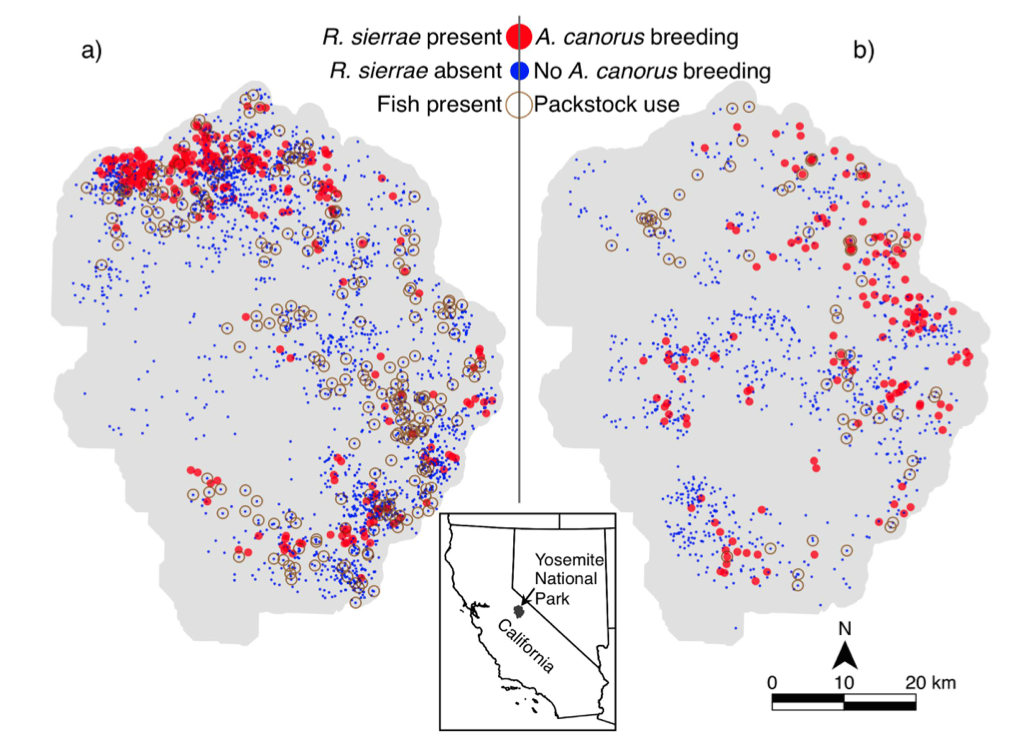
\includegraphics[height = 0.75\textheight]{fig/toadmap.png}
\end{center}
\end{figure}


\tiny
J. R. Matchett, Philip B. Stark, Steven M. Ostoja, Roland A. Knapp, Heather C. McKenny, Matthew L. Brooks,
William T. Langford, Lucas N. Joppa, and Eric L. Berlow. Detecting the influence of rare stressors on rare species in Yosemite National Park using a novel stratified permutation test.
Scientific Reports, 5: 10702, June 2015.
}

\frame{
\frametitle{Toads and Packstock}

\begin{itemize}
\itemsep10pt
\item Response is binary: did toads breed in the meadow or not?
\item Treatment is continuous: average or maximum packstock nights in each meadow
\item Prediction: probability of toad presence according to meadow characteristics
\item Test statistic: within-stratum absolute value of correlation between treatment and residuals, averaged over strata
\end{itemize}
}


\frame{
\frametitle{Toads and Packstock}
Intensity of packstock use appears to be \textbf{weakly correlated} with toad presence. The correlation is not significant.
 
\begin{figure}[htbp]
\begin{center}
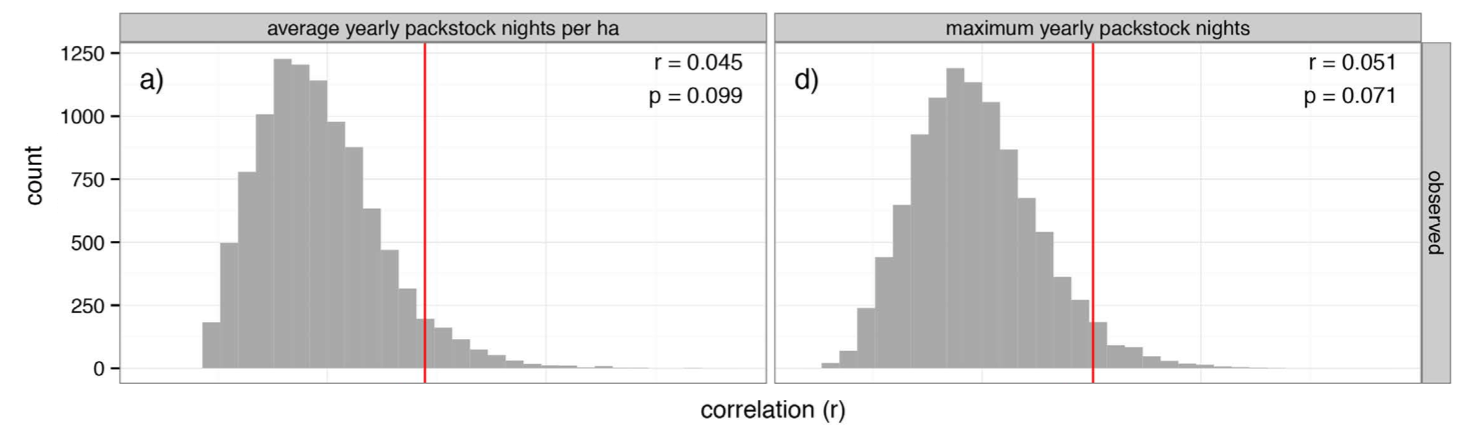
\includegraphics[width = \textwidth]{fig/toad_results.png}
\end{center}
\end{figure}

\vfill

\tiny
J. R. Matchett, Philip B. Stark, Steven M. Ostoja, Roland A. Knapp, Heather C. McKenny, Matthew L. Brooks,
William T. Langford, Lucas N. Joppa, and Eric L. Berlow. Detecting the influence of rare stressors on rare species in Yosemite National Park using a novel stratified permutation test.
Scientific Reports, 5: 10702, June 2015.
}




\subsection[Salt and Mortality]{Salt and Mortality}

\frame{
\frametitle{Salt}

\begin{itemize}
\itemsep10pt
\item There is a major campaign by the World Health Organization (WHO) to reduce salt consumption worldwide \citep{WHO}
\item WHO assumes a causal pathway between eating salt and mortality. Main sources of evidence that salt is bad come from observational studies on hypertension \citep{Intersalt}
\item \textbf{Goal:} test whether changes in sodium intake are associated with changes in life expectancy, after controlling for other major predictors of health.
\end{itemize}


}


\frame{
\frametitle{Salt}
An example of faulty analysis of salt and morbidity: \\
\vspace{10pt}
After excluding indigenous tribes (red points) from the sample, the association between salt and hypertension \textbf{changes sign} \citep{FreedmanPetitti}.



\begin{center}
\begin{figure}[htbp]
\begin{center}
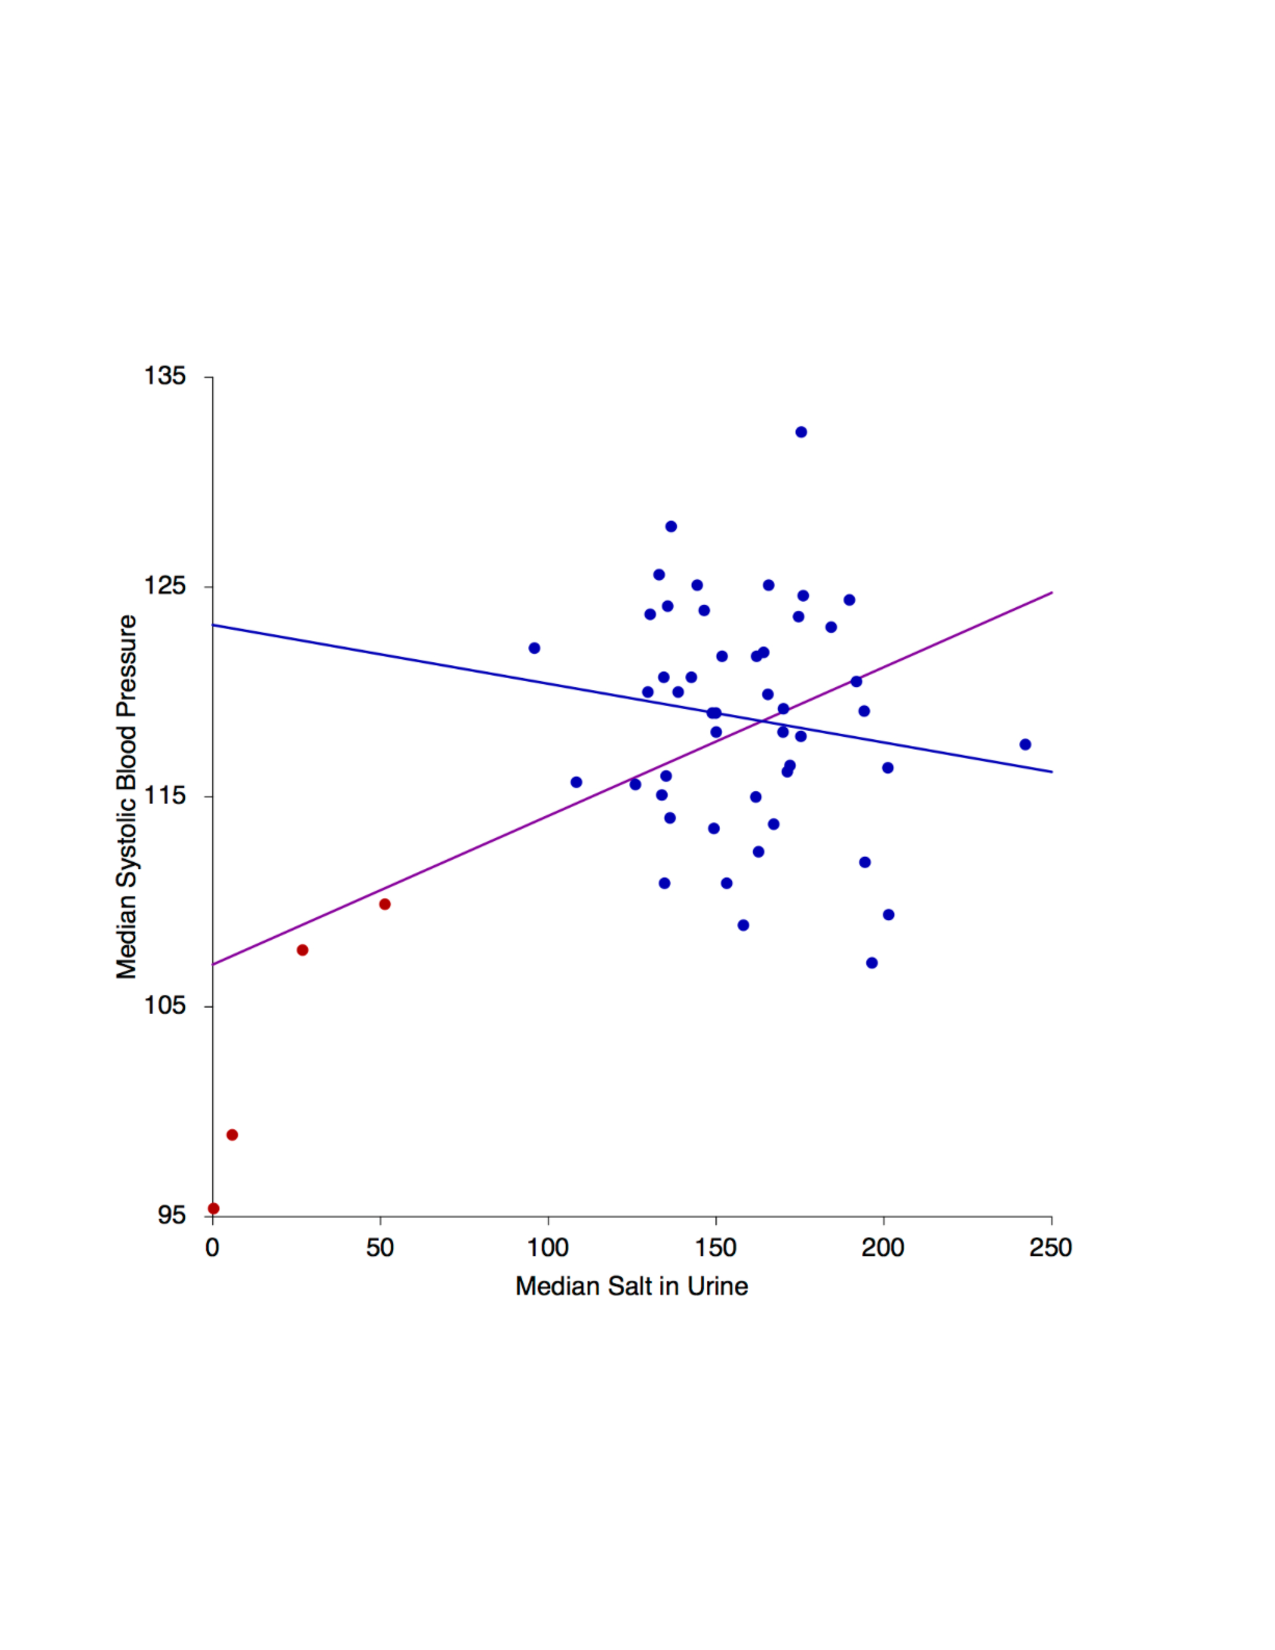
\includegraphics[height = 0.6\textheight]{fig/freedmanplot.pdf}
\end{center}
\end{figure}
\end{center}
}

\frame{
\frametitle{Salt}

\begin{itemize}
\itemsep10pt
\item Response is continuous: life expectancy at age 30
\item Treatment is continuous: mean daily sodium intake
\item Prediction: life expectancy at age 30, given alcohol consumption per capita per year, cigarettes per capita per year, and per capita GDP using random forests
\item Test statistic: Pearson correlation between treatment and residuals
\item All variables are differenced from 1990 to 2010 to control for baseline levels. Analyses are separate for males and females.
\end{itemize}
}



\frame{
\frametitle{Salt}
Sodium consumption appears to be 
\begin{itemize}
\item \textbf{uncorrelated} with life expectancy for males 
\item \textbf{positively correlated} with life expectancy for females
\end{itemize}

\begin{center}
\begin{figure}[htbp]
\begin{center}
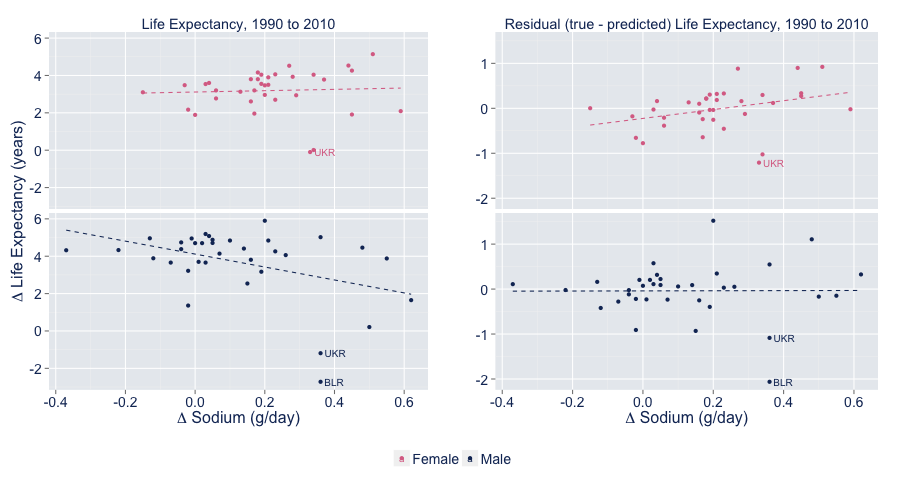
\includegraphics[width = 0.9\textwidth]{fig/sodium_lifeexp.png}
\end{center}
\end{figure}
\end{center}
}


\section[Conclusions]{Conclusions}

\frame{
\frametitle{Conclusions}
\begin{itemize}
\itemsep20pt
\item We've developed a novel nonparametric test for treatment effects in observational studies.
\item Model-based matching is more flexible than traditional methods: it has power to detect non-constant effects and can be used when treatment is non-binary.
\item Stronger assumptions are needed to assert causation instead of just association.
\end{itemize}

}

\frame
{
  \frametitle{Future Directions}
\begin{center}
\begin{itemize}
\itemsep20pt
\item Do different test statistics give greater power?  Under what conditions?
\item What is the optimal way to stratify?
\item How to quantify uncertainty -- standard errors and confidence intervals?
\end{itemize}
\end{center}
}




\begin{frame}
\frametitle{References}
\tiny
\bibliographystyle{plainnat}
\bibliography{refs}
\itemize
\end{frame}


\end{document}
